
\subsection{Web Content}
\label{sec:assessment_3rdpartydep}

The crawl succeeded for 1,517 of 1,988 input domains (76.3\%). Success requires a 2xx/3xx HTTP status and a non-blank screenshot in the initial normal load. The successful domains by sector are: Government: 331/460 (72.0\%); University: 496/677 (73.3\%); Bank: 355/452 (78.5\%); Newspaper: 335/399 (84.0\%). Reasons for failed page-loads include navigation timeouts (264 cases), blank screenshots (128 cases), and HTTP 4xx responses (62 cases, including 54 HTTP 403 responses). Although these failed page-loads do not affect sector coverage, all 17 Lithuanian government domains returned HTTP 403 responses. Consequently, the web-content sovereignty score is unavailable for this country-sector combination. Future measurements from country-local vantage points could help address this limitation. We evaluate web content dependence at four levels: the share of outside EU requests, the affected resource types, the destination organizations of requests, and the observable page-level effect when requests outside EU are blocked. 

\paragraph{Request Share}
Figure~\ref{fig:hosting-sovereignty-bars} (c) shows while a larger share of requests remain in the EU, only a small share of domains is providing web content without non-EU dependencies.
Overall, 1,367 domains (90.1\%) contact at least one ASN/operator classified outside the EU, and these requests account for 56.0\% of all observed blocked-run request events. Government and university pages keep most requests inside EU-classified infrastructure: mean per-domain in-EU request shares are 65.7\% and 69.4\%, respectively. Banks are split more evenly at 49.7\%, while newspapers are the outlier at 40.5\%. Fully autonomous pages are rare. Only 23.0\% of government domains avoid outside-EU ASNs/operators entirely; the corresponding shares are 10.1\% for universities, 4.5\% for banks, and 2.4\% for newspapers.

\paragraph{Resource Types}
Figure~\ref{fig:3presources} shows differences across request types, ranked by the share of domains that rely on each resource type. Sector-level differences are visible, with government and university pages hosting a larger share of resources within the EU. Image, script, and stylesheet requests are the dominant resource loads across the investigated pages. To highlight non-content resources that introduce dependencies on infrastructure outside the EU, we report their prevalence on government websites: Google Tag Manager appears on 67 government domains (20.2\%), Google Analytics on 18 (5.4\%), and Google Fonts and CSS on 83 (23.3\%). Other dependencies include jsDelivr CDN libraries on 28 government domains (8.5\%), Cloudflare cdnjs on 23 (6.9\%), Facebook SDK/event scripts on 14 (4.2\%), and Cloudflare Insights on 9 (2.7\%). The crawl also shows the use of Matomo/Piwik on 71 government domains (21.5\%), indicating that some governments instead choose analytics stacks that can be EU-hosted or self-hosted.  

\begin{figure}
    \centering
    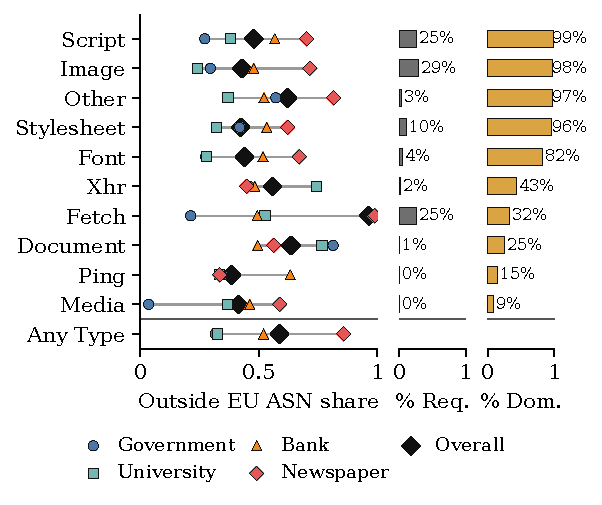
\includegraphics[width=0.8\linewidth]{resource_type_location_probability_by_sector_barcols_sorted_dom_doc.pdf}
    \caption{Share of outside-EU ASNs on classified requests by browser resource type and sector.}
    \label{fig:3presources}
\end{figure}



\paragraph{Non-EU Request Destinations}
Across all sectors, 70.5\% of domains load resources from Google-operated ASNs, 49.0\% from Cloudflare, 37.9\% from Amazon, 19.3\% from Fastly, and 13.8\% from Microsoft. By request volume, Amazon accounts for the largest share among these operators, with 32.3\% of classified resource requests, followed by Cloudflare (12.2\%), Akamai (5.1\%), Google (3.7\%), Microsoft (3.0\%), and Fastly (2.6\%). This concentration is strongest among newspapers and universities, but it is also visible on government websites: 41.7\% of government domains load resources from Google-operated ASNs, 31.4\% from Cloudflare, and 29.0\% from Amazon.

\paragraph{Request Blocking}
We next evaluate the effect of blocking requests classified as outside the EU to assess their contribution to page content. Many pages retain their main visual content: mean visual loss is 7.4\% for government websites, 8.5\% for universities, 7.3\% for banks, and 11.9\% for newspapers. Structural changes are larger, with HTML loss reaching 19.1\% for banks and 20.4\% for newspapers. This suggests that outside-EU resources often support page modules that are not visually dominant, such as scripts, tracking, advertising, and consent components. Under restrictions on non-EU services, the main page content would therefore often remain visible, provided that primary hosting and essential delivery infrastructure remain under EU jurisdiction.